% THIS IS SIGPROC-SP.TEX - VERSION 3.1
% WORKS WITH V3.2SP OF ACM_PROC_ARTICLE-SP.CLS
% APRIL 2009
%
% It is an example file showing how to use the 'acm_proc_article-sp.cls' V3.2SP
% LaTeX2e document class file for Conference Proceedings submissions.
% ----------------------------------------------------------------------------------------------------------------
% This .tex file (and associated .cls V3.2SP) *DOES NOT* produce:
%       1) The Permission Statement
%       2) The Conference (location) Info information
%       3) The Copyright Line with ACM data
%       4) Page numbering
% ---------------------------------------------------------------------------------------------------------------
% It is an example which *does* use the .bib file (from which the .bbl file
% is produced).
% REMEMBER HOWEVER: After having produced the .bbl file,
% and prior to final submission,
% you need to 'insert'  your .bbl file into your source .tex file so as to provide
% ONE 'self-contained' source file.
%
% Questions regarding SIGS should be sent to
% Adrienne Griscti ---> griscti@acm.org
%
% Questions/suggestions regarding the guidelines, .tex and .cls files, etc. to
% Gerald Murray ---> murray@hq.acm.org
%
% For tracking purposes - this is V3.1SP - APRIL 2009

\documentclass{acm_proc_article-sp}

\begin{document}

\title{On the Ground Validation of Online Diagnosis with Twitter and Medical Records}


%
% You need the command \numberofauthors to handle the 'placement
% and alignment' of the authors beneath the title.
%
% For aesthetic reasons, we recommend 'three authors at a time'
% i.e. three 'name/affiliation blocks' be placed beneath the title.
%
% NOTE: You are NOT restricted in how many 'rows' of
% "name/affiliations" may appear. We just ask that you restrict
% the number of 'columns' to three.
%
% Because of the available 'opening page real-estate'
% we ask you to refrain from putting more than six authors
% (two rows with three columns) beneath the article title.
% More than six makes the first-page appear very cluttered indeed.
%
% Use the \alignauthor commands to handle the names
% and affiliations for an 'aesthetic maximum' of six authors.
% Add names, affiliations, addresses for
% the seventh etc. author(s) as the argument for the
% \additionalauthors command.
% These 'additional authors' will be output/set for you
% without further effort on your part as the last section in
% the body of your article BEFORE References or any Appendices.

\numberofauthors{3} %  in this sample file, there are a *total*
% of EIGHT authors. SIX appear on the 'first-page' (for formatting
% reasons) and the remaining two appear in the \additionalauthors section.
%
\author{
% You can go ahead and credit any number of authors here,
% e.g. one 'row of three' or two rows (consisting of one row of three
% and a second row of one, two or three).
%
% The command \alignauthor (no curly braces needed) should
% precede each author name, affiliation/snail-mail address and
% e-mail address. Additionally, tag each line of
% affiliation/address with \affaddr, and tag the
% e-mail address with \email.
%
% 1st. author
\alignauthor
Todd Bodnar\titlenote{Corresponding author}\\
       \affaddr{Pennsylvania State University}\\
\affaddr{Department of Biology}\\
       \affaddr{University Park, PA 16802}\\
       \email{tjb5215@psu.edu}
% 2nd. author
\alignauthor
Maybe Conrad, Maybe Vicky
% 3rd. author
\alignauthor
Marcel Salath\'e\\
       \affaddr{Pennsylvania State University}\\
\affaddr{Department of Biology}\\
       \affaddr{University Park, PA 16802}\\
       \email{salathe@psu.edu}
}

\maketitle
\begin{abstract}
This is an abstract
\end{abstract}

% A category with the (minimum) three required fields
%\category{I.6.4}{Simulation and Modeling}{Model Validation and Analysis}
\category{I.2.1}{Artificial Intelligence}{Applications and Expert Systems}[Medicine and Science]
%A category including the fourth, optional field follows...
%\category{D.2.8}{Software Engineering}{Metrics}[complexity measures, performance measures]

\terms{Experimentation, Validation}

\keywords{Twitter, Validation, Digital Epidemiology, Remote Diagnosis} % NOT required for Proceedings

\section{Introduction}
Digital epidemiology \(\to\) novel disease detection mechanisms.

Validation of this idea is important, but not done.

Pull med info of individuals professionally diagnosed with ILI and their twitter accts. Compare old methods. Suggest some new things.

\section{Related Work}

People with issues \cite{Bodnar:2013we,Butler:2013uh,Lamb:2013to} also plos paper!

Most work to this point considers finding messages in tweets (i.e. ``I'm sick'') or in keyword frequencies. 

Keyword \cite{Culotta:2010hx,Goel:2010jf}

Tweet classification \cite{Culotta:2010hx,Lamb:2013to,Salathe:2011gr}

\section{Data Collection}
\subsection{Medical Records}
\subsection{Twitter Records}
Screen names taken from med records, total of 119 individuals gave us twitter handle. Threw out 15 accounts because either not legit, banned, or blocked for total of 104 seed accounts.

Tweets collected through twitter timeline query. API limits to most recent 3000 tweets per account. Two cases where this was an issue, both thrown out (users that consistently tweet multiple times per hour, barely any back data available. oddly twitter site does not give accurate tweet count.) Simple loop through every account. Once first pass, process by pulling any new tweets from user that has longest time since last query. 

Pulled all friends / followers from accounts. Repeated tweet pull from these. Again, process oldest first.

\section{Signal Detection}
\subsection{Event Based Signals}

In this section, we consider diagnosis based on classifying an individual tweet's content as either about ILI or not. We begin by dividing the tweets into two sets: tweets that were posted the same month that a user was sick, and tweets that were posted other times. We find a total of 1609 (out of Y) tweets from X users in the first category.

First we go the route of AUTHOR and AUTHOR by defining a set of keywords that are positive signals of influenza. We choose KEYWORD LIST as our set of keywords. Of the 999 keywords, we find a significantly higher amount of 999 keywords during months when the user had ILI. (See table X). Additionally, we use METHOD to automatically find keywords with a significant effect (See table Y). In both of these cases, we preprocess the data by tokenizing the text with the regex "REGEX", remove stop words\footnote{Stop words taken from HERE}, perform iterated levins stemming and ignoring case. For each keyword \(x\), we define an individual as sick on month \(m\) if their Twitter stream contains \(x\) atleast one time. We find this method to correctly classify users \% of the time. (See tables \ref{tab:tweet_keyword_expert_confusion} and \ref{tab:tweet_keyword_algorithm_classified_confusion})


Finally, we hand rate all 1609 tweets that were posted by individuals during the time of their illness for information regarding the user's health. Additionally we sample a randomly selected set of 1609 tweets from times when the users did not have ILI as a control. We find 58 tweets from 17 (\(17/119 = 14.29\%\)) of the individuals in our study that are about them being sick. We also find x tweets from y/Z of individuals about ILI during times when they did \textit{not} have ILI. Thus we would expect a health monitoring system based off of tweet classification to operate at \% accuracy. (See table \ref{tab:tweet_classified_confusion})


\begin{table}
\centering
\begin{tabular}{|c|c|c|} \hline
Sick&Not Sick&\ \\ \hline
1 & 2& Sick\\ \hline
3 & 4  & Not Sick\\
\hline\end{tabular}
\caption{Confusion matrix of a classifier based on keywords from a domain expert. Rows are of true values, columns are of predicted values.}
\label{tab:tweet_keyword_expert_confusion}
\end{table}

\begin{table}
\centering
\begin{tabular}{|c|c|c|} \hline
Sick&Not Sick&\ \\ \hline
1 & 2& Sick\\ \hline
3 & 4  & Not Sick\\
\hline\end{tabular}
\caption{Confusion matrix of a classifier based on keywords derived from an algorithmic aproach. Rows are of true values, columns are of predicted values.}
\label{tab:tweet_keyword_algorithm_classified_confusion}
\end{table}

\begin{table}
\centering
\begin{tabular}{|c|c|c|} \hline
Sick&Not Sick&\ \\ \hline
17 & 102 & Sick\\ \hline
3 & 4  & Not Sick\\
\hline\end{tabular}
\caption{Confusion matrix of a Tweet-Classification based diagnosis system. Rows are of true values, columns are of predicted values.}
\label{tab:tweet_classified_confusion}
\end{table}

\subsection{Frequency Based Signals}

Look at changes in behaviour based on illness. May have signal even if no  relevant messaging.

In each user, take months when they did tweet, apply normalization (val - min)/(max-min)

Build distributions of months before, during, and after illness. Compare distributions. Try paired / unpaired

Fail to find sig difference between three sets \(\to\) comment on benefits of this.

Try anomoly detection...


%\begin{figure} %need to redo
%\centering
%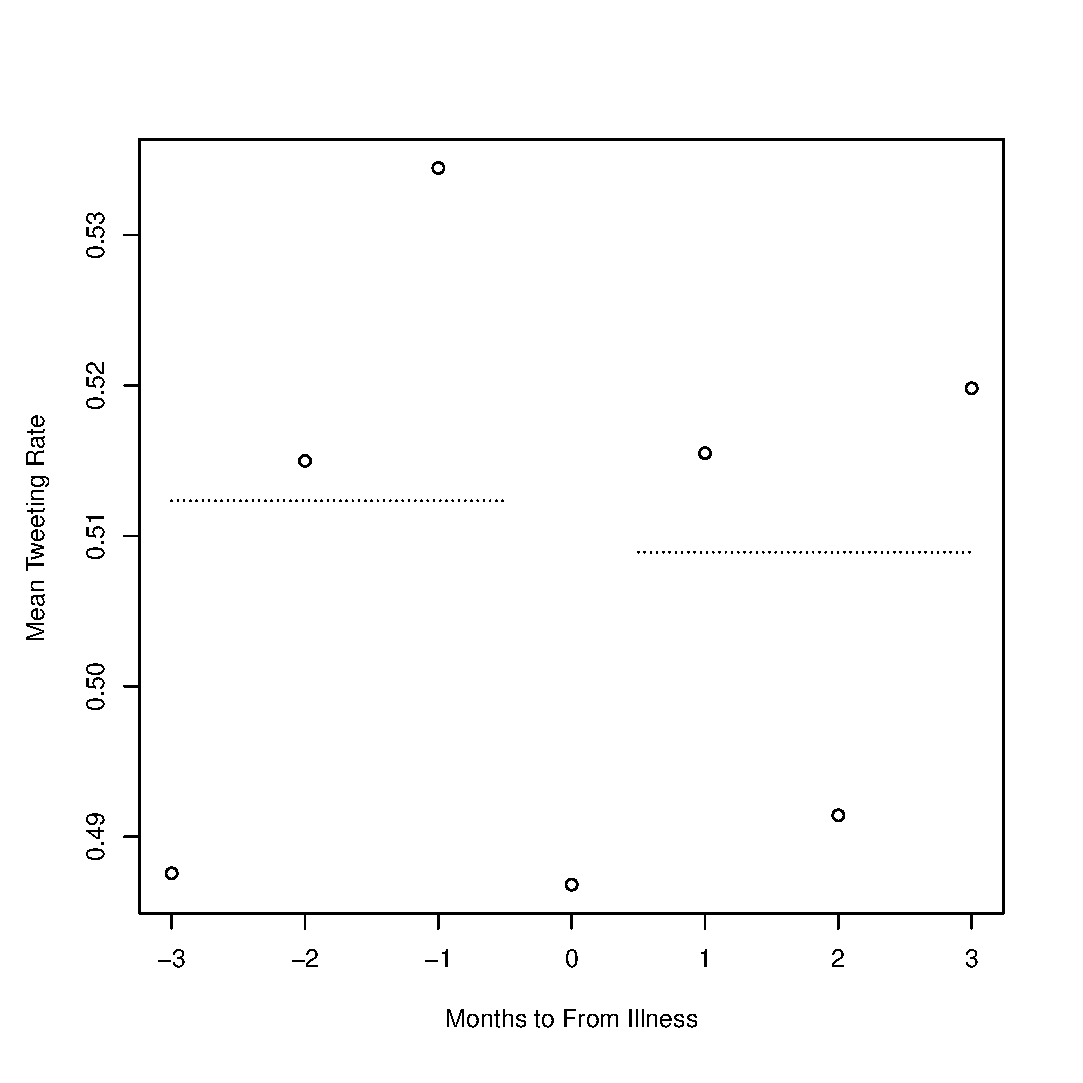
\includegraphics[width=0.5\textwidth]{figs/meanFrequencies.eps}
%\caption{The frequency of tweeting behaviour of individuals in the months before, during and after an illness. Users significantly (check) decrease their rate of tweeting during the time that they had influenza. Dashed lines indicate the mean rate for the three months before / after the illness. (Todo: check significance)}
%\label{fig:mean_freq}
%\end{figure}





\subsection{Network Based Signals}

Preliminary idea. Cascade effects causing echoes on social network. Also consider friends becoming ill around same time. Check @ tag

\section{Analysis}

\section{Conclusions}

%\begin{thebibliography}{1}
%\bibitem{Ford:1956vc}
%L. R. Ford and D. R. Fulkerson. \newblock{Maximal Flow through a Network}. \newblock{\em Canadian Journal of Mathematics}, 8(3):399-404, 1956.
%\end{thebibliography}



%@article{Ford:1956vc,
%author = {Ford, L R and Fulkerson, D R},
%title = {{Maximal Flow through a Network.}},
%journal = {Canadian Journal of Mathematics},
%year = {1956},
%pages = {399--404}
%}


%
% The following two commands are all you need in the
% initial runs of your .tex file to
% produce the bibliography for the citations in your paper.
\bibliographystyle{abbrv}
\bibliography{library}  % sigproc.bib is the name of the Bibliography in this case
% You must have a proper ".bib" file
%  and remember to run:
% latex bibtex latex latex
% to resolve all references
%
% ACM needs 'a single self-contained file'!
%
%APPENDICES are optional
%\balancecolumns

\balancecolumns
% That's all folks!
\end{document}
